\documentclass[12pt, letterpaper]{article}
\usepackage[titletoc,title]{appendix}
\usepackage{color}
\usepackage{booktabs}
\usepackage{caption}
\newcommand\fnote[1]{\captionsetup{font=small}\caption*{#1}}

\usepackage[usenames,dvipsnames,svgnames,table]{xcolor}
\definecolor{dark-red}{rgb}{0.75,0.10,0.10} 
\usepackage[margin=1in]{geometry}
\usepackage[linkcolor=dark-red,
			colorlinks=true,
			urlcolor=blue,
			pdfstartview={XYZ null null 1.00},
			pdfpagemode=UseNone,
			citecolor={dark-red},
			pdftitle={Face of Crime in Prime Time}]{hyperref}
\usepackage{multibib}
\usepackage{geometry} % see geometry.pdf on how to lay out the page. There's lots.
\geometry{letterpaper}               % This is 8.5x11 paper. Options are a4paper or a5paper or other... 
\usepackage{graphicx}                % Handles inclusion of major graphics formats and allows use of 
\usepackage{amsfonts,amssymb,amsbsy}
\usepackage{amsxtra}
\usepackage{natbib}
\usepackage{verbatim}
\setcitestyle{round,semicolon,aysep={},yysep={;}}
\usepackage{setspace}		     % Permits line spacing control. Options are \doublespacing, \onehalfspace
\usepackage{sectsty}		     % Permits control of section header styles
\usepackage{lscape}
\usepackage{fancyhdr}		     % Permits header customization. See header section below.
\usepackage{url}                 % Correctly formats URLs with the \url{} tag
\usepackage{fullpage}		     %1-inch margins
\usepackage{multirow}
\usepackage{rotating}
\setlength{\parindent}{3em}
\usepackage{subcaption}
\usepackage[T1]{fontenc}
\usepackage{bm}
\usepackage{libertine}

\usepackage{chngcntr}

\title{\Large{The Face of Crime in Prime Time:\\ Evidence from Law and Order}\footnote{Data and scripts behind the analysis presented here can be downloaded at: \url{http://github.com/soodoku/face_of_crime}.}}

\author{Gaurav Sood\thanks{Gaurav can be reached at \href{mailto:gsood07@gmail.com}{\footnotesize{\texttt{gsood07@gmail.com}}}} \and Daniel Trielli\thanks{Daniel is a professional journalist. He can be reached at: \href{mailto:dtrielli@gmail.com}{\footnotesize{\texttt{dtrielli@gmail.com}}}}\vspace{.5cm}}

\date{\vspace{.5cm}\normalsize{\today}}

\begin{document}
\maketitle

\begin{center}
\vspace{.5cm}\textbf{NB:} Preliminary draft. Please do not cite without permission.\vspace{1.5cm}
\end{center}

\begin{comment}

setwd(paste0(basedir, "face_of_crime/ms"))
tools::texi2dvi("face_of_crime.tex", pdf=TRUE, clean=TRUE) 
setwd(basedir)

\end{comment}


\begin{abstract}
\noindent Race, gender, and crime are inextricably linked in people's minds. Television programming is thought to strongly influence how they are linked. We investigate the extent to which popular television programming perpetuates stereotypical linkages by tallying the race and gender of perpetrators and victims in three popular series of the most successful criminal procedural franchise on television---Law \& Order. Using data from a census of the shows from aired seasons of \textit{Special Victims Unit} and \textit{Criminal Intent} series, and data from seven seasons of the \textit{Original} series, we find that whites and women are overrepresented (and blacks and men underrepresented), both as victims and as perpetrators. There is some expected variation across the series---the proportion of female victims in \textit{Special Victims Unit} is considerably higher than the other two series---and no discernible trend over time for either race or gender for either victims or perpetrators. 
\end{abstract}
\clearpage
\doublespace

Among the most foundational of the cognitive biases is the tendency to overweight accessible information \citep{tversky1973availability, iyengar2010news, iyengar1990accessibility}. For instance, one of the reasons comparisons with peers weigh heavily in people's assessments of their own lives is because information about peers is much more readily available. Given the importance of accessible information in attitude formation and decision making, what is covered on television has been a natural focus of inquiry. 

One particularly important topic in that inquiry has been whether television programming propagates aversive racial stereotypes. Common longstanding aversive stereotypes about blacks are that they are lazy, poor, unintelligent and violent \citep{katz1933racial}. And much research shows that such stereotypes shape political attitudes \citep{sniderman1995scar, hurwitz1997public, peffley1997racial, dixon2006psychological} and affect economic behavior \citep{bertrand2004emily}. 

Vitally, research also suggests that these stereotypes are correlated with exposure to television programming \citep{busselle2002television, entman2001black, armstrong1992tv}. For instance, exposure to television news is correlated with the extent to which college students endorse that blacks are lazy \citep{busselle2002television}. Similarly, \citet{armstrong1992tv} find that college students who consume more television news were more likely to believe that blacks had lower socio-economic outcomes. (Albeit, ``TV drama exposure was associated with beliefs that Black Americans had a relatively higher socio-economic standing.'') A comprehensive study of how blacks are portrayed in the media by \citet{entman2001black} reached similar conclusions---it found that nonfictional portrayals of African Americans were associated with negative stereotypes of blacks, including, for instance, the perception that they are hostile.

Given the longstanding concern, numerous researchers have studied how blacks are covered on various television programs \citep[for e.g.,][]{entman2001black, eschholz2004images}. One particular focus of the effort---given the stereotype of blacks as violent and criminal, and given the impact such stereotypes may have on policy consequential attitudes related to punitiveness---has been on describing the extent to which blacks are overrepresented as criminals, especially as violent criminals. 

Studies on the extent to which blacks are overrepresented in news or other programming about crime suggest that the bias is generally small but fairly variable---some studies document a modest anti-black bias in some news programs in some areas of the country \citep{gilliam1996crime}, while others document a large anti-white bias (when compared to criminal arrest data, which are likely biased in favor of whites) \citep{chiricos2002racial, dixon2000overrepresentation, eschholz2004images} (see Table \ref{tab:lit}). 

% latex table generated in R 3.3.1 by xtable 1.8-2 package
% Wed Sep 21 08:33:25 2016
\begin{table}[!htb]
\centering
\caption{Racial Distribution of Perpetrators and Victims on Various Television Shows} 
\label{tab:lit}
\begingroup\tiny
\begin{tabular}{p{0.1\textwidth}p{0.1\textwidth}p{0.1\textwidth}p{0.55\textwidth}p{0.12\textwidth}}
  \hline
Region Covered & Time frame & Media & Key Relevant Findings & Citation \\ 
  \hline
Hampton Roads, Virginia & Jan. 3-31, 2011 & Local TV News & Perpetrators: 50.7\% Blacks (Violent Crime), 75\% Whites (White Collar Crime),  75.9\% Blacks (General Crime) (Graph 4) 

Victims: 78.3\% White (Violent Crime), 82.1\% Whites (General Crime) (Graph 5) & \citet{leadbleed2011} \\ 
  National & 1994--1997, 2000 & Network News & Perpetrators: 

All Crime: 71\% White (vs. 68\% in Uniform Crime Reports),  27\% Blacks (vs. 30\% in Uniform Crime Reports) (Table 4)

Violent Crime: 48\% White (vs. 56\% in Uniform Crime Reports), 38\% Blacks (vs. 42\% in Uniform Crime Reports) (Table 5)

Victims:
All Crime: 51\% White (vs. 28\% in Uniform Crime Reports),  30\% Blacks (vs. 48\% in Uniform Crime Reports) (Table 6) & \citet{dixon2003portrayal}  \\ 
  National & 2002--2003 & Local TV News & Perpetrator (All Crime): 26.82\% White, 21.06\% Black, 42.27\% Not Indicated 

Victim (All Crime): 27.88\% White,  9.24\% Black, 56.97\% Not Indicated (Table 1) & \citet{bjornstrom2010race} \\ 
  National & 2000--2001 & NYPD Blue and Law and Order & NYPD Blue: 

Offender:  50\% Whites (vs. 68\% in Uniform Crime Reports),  38\% Blacks, 11\%

Violent Off./Sus. 43\% (black) 46\% (white) 10\%  

Law and Order Figures don't add up to 100. (Table 1) & \citet{eschholz2004images} \\ 
  Washington, D.C. & May and June 2005 & Local TV News & Perpetrators: 
Violent Crime: 9\% Whites, 32\% Blacks, 51\% Unrevealed 

Non-violent Crime: 14\% Whites, 29\% Blacks, 50\% Unrevealed 

Victims: 

Violent Crime: 15\% White,  10\% Blacks, 72\% Unrevealed 

Non-violent Crime: 3\% White,  7\% Blacks, 83\% Unrevealed & \citet{gross2006covering} \\ 
  Los Angeles & 1995--1996 & Local TV News & All Perpetrators: 37\% Black (versus 21\% in California Department of Justice Criminal Profile or CDJCP), 21\% (versus 28\% in CDJCP) (Table 4) 

Felons: 44\% Black (versus 25\% in CDJCP), 18\% (versus 23\% in CDJCP) (Table 5) & \citet{dixon2000overrepresentation} \\ 
  Los Angeles & 1993--1994 & Local TV News (KABC) & No commensurate numbers, except: 40\% where race identified (purportedly across all crime stories). Where race identified in violent crime stories: 45\% White and in non-violent crime: 75\% white. 

Blacks actual crime rate: 2.8 * share of population. Coverage: 3.2 * share of population. (Assuming the coverage is estimated as percentage where race identified and not as percentage of total mentions) (Figure 2) 

Non-violent crime: Whites overrepresented by nearly 400\% (see Figure 3) & \citet{gilliam1996crime} \\ 
  Orlando & 1998 & Local TV News & All Crime: 18\% Black (Versus 42\% Arrest Rate),  65\% White (Versus 58\% Arrest Rate) (Table  3)

Violent Crime: 20\% Black (Versus 49\% Arrest Rate), 61\% White (Versus 51\% Arrest Rate)(Table  3) & \citet{chiricos2002racial} \\ 
   \hline
\end{tabular}
\endgroup
\end{table}


In this paper, we add to this body of work. We tally the gender and race of criminals and victims depicted in three popular series of the criminal procedural, Law \& Order. Compared to arrest records, victim survey data, and population demographics, all three series overrepresent whites and women, both as criminals and as victims. Data show that the share of violent crime depicted in the series is also exceedingly high.

\section*{Learning from Television}

We are constantly learning from our environment, though not always effortfully. One salient place we learn from is the mass-media. For instance, local news, the most common kind of news programming that people tune into \citep{pew2004}, carries lots of episodic coverage of violent crime \citep[see, for instance,][]{gross2006covering, klite1997local}. And watching multiple daily reports of violent crime may cause them to think that violent crime is `common'---a phrase that the person internally maps to a number much larger than actual incidence of violent crime.

Similar, though more subtle, mechanism likely holds when someone watches one of the tens of hundreds of crime dramas on television. A person watching a crime drama, aware of its fictional nature, may still inadvertently think that the drama accurately `mirrors' society. This inference may be encouraged by prior interpretation and acceptance of imprecise flawed statements such as 'art reflects life' as true. Increasingly common mass-media tropes such as realism in depiction, and explicit statements designed to cue realism, may also increase the chances that people take fictional portrayals as reasonably accurate depictions of reality. As a case in point, all Law \& Order \textit{Special Victims Unit} series episodes start with the statement: ``...In New York City, the dedicated detectives who investigate these vicious felonies are members of an elite squad known as the Special Victims Unit. These are their stories.'' It is not unreasonable to assume that someone listening to the statement may come to think that the crimes covered in the drama represent a broad, perhaps representative, set of all ``sexually based crimes.''

Besides the extent of crime and what kind of crime is prevalent, people may also learn associations between kinds of people and criminal activity, especially when people involved are (superficially) distinctive---say, in the color of their skin. The logic goes that if certain kinds of people are frequently shown as perpetrators of crime, people may come to believe that as large a share of perpetrators belongs to that group. By the same token, over-representation of certain groups as victims may promote misleading views of what populations are the most vulnerable to crime.

\section*{Data and Measurement}
The data are from three Law \& Order series: the Original Law \& Order series (Original), Law \& Order: Special Victims Unit (SVU), and Law \& Order: Criminal Intent (CI). All the three shows are police procedurals set in New York City. CI, which ran between 2001--2011, purportedly follows detectives of the `Major Case Squad,' a division of the New York Police Department (NYPD) focused on solving major crimes against rich, famous, or important people. Meanwhile SVU, which has been on television since 1999, purportedly follows detectives of the NYPD division devoted to handling ``sexually based offenses,'' the `Special Victims Unit.'

All three shows have enjoyed great success. The Original Law \& Order is the longest running scripted US prime time TV series on a major broadcast network, while SVU is the longest running scripted non-animated US prime time TV series currently on air. Through its run, CI drew an average of 9.3M people, Original an average of 10.2M, and SVU an average of 11.81M.\footnote{Based on data assembled by Austin Ogilvie at \href{https://github.com/hernamesbarbara/law_and_order}{https://github.com/hernamesbarbara/law\_and\_order} from Wikipedia and TV.com.}

For the original series, we only have data from Seasons 1 and 2 (1990--1991) and Seasons 16--20 (2005--2010).\footnote{The choice of the seasons is a reflection of what was available on streaming on Amazon Instant as of July, 2016.} In all, we have data from 151 shows. For CI, we have data on all 194 shows across all 10 seasons, spanning 2001--2011. And for SVU, we have data on all the 386 shows that were part of the sixteen seasons spanning 1999--2015. In all, across the three series, we have data from 731 shows, featuring over 1500 characters that were victims of crime, and over 1100 characters that committed a crime. We coded the race and gender of almost all of the characters whose race and gender was identified. 

We defined criminals as characters who were clearly indicated as guilty; our definition includes characters not convicted or even indicted for a crime. In line with the law, active instigators and financiers of crime were also coded as criminals. We marked attempted crimes as such. Since the focus is on `major' crimes, we decided not to include infractions such actions such as failing to comply with court orders. 

We coded victims' and criminals' race as white, black, Asian, or Hispanic, following the general census guidelines.\footnote{\url{http://www.census.gov/topics/population/race/about.html}} Characters of Middle-Eastern descent were coded as white, but a note marking their specific background is included in the data file. And under `Hispanics,' we included non-Hispanic Latinos such as Brazilians.

In addition to data on race and gender from the shows, we collected data on a few baselines. In particular, from the 1990, 2000, and 2010 census, we collected data on the proportion of whites, blacks and men in the US and in the NYC. Like \citet{dixon2000overrepresentation}, from Federal Bureau of Investigation's Uniform Crime Report (UCR), we collected data on percentage of blacks, whites and men arrested for all crime, violent crime, and sexually based crime. Lastly, from the Bureau of Justice Statistics' National Crime Victimization Survey (NCVS) \citep{powers2016national, victimization1998national}, we collected data on race and gender of victims of crime.  

The UCR data on percentage of people arrested by race and sex covers 1995 to 2014. (Only preliminary data is available for 2015. For now, it does not include data on race.) In UCR, race is divided into White, Black or African American, American Indian or Alaska Native, Asian, and Native Hawaiian or Other Pacific Islander. The totals in those categories include non-Hispanics and Hispanics. Specific data on Hispanic background only began to be gathered in 2013. 

In UCR, 28 types of crimes are split into two categories: Violent Crime and Property Crime. Violent Crime includes murder and non-negligent manslaughter, rape, robbery, and aggravated assault. And Property Crime includes burglary, larceny-theft, motor vehicle theft, and arson. We collected data on the percentage of people arrested by race (white and black) and gender (male) for all crimes, violent crimes, as well as arrested for three of the most common offenses shown in the Law \& Order shows: homicides, rapes, and assaults.

Victim data from NCVS covers the period between 1993--2014. Racial data in the NCVS can be gathered both with Hispanics included in the racial totals or not. We collected data on both, but focused on the data that more closely matches the FBI methodology and does not separate out Hispanics.

Like the UCR, the NCVS has data on specific types of crime that is aggregated into categories. In NCVS, however, the categories are \textit{Violent Victimization} and \textit{Serious Violent Victimization}. Both account for victims of rape, sexual assault, and robbery. \textit{Violent victimization}, however, tallies all types of assault, while \textit{Serious Violent Victimization} only tallies aggravated assaults. Therefore, \textit{Serious Violent Victimization} is the closest to the \textit{Violent Crimes} category in the UCR. Hence, we use data from that category and for two specific offenses: rape/sexual assault and aggravated assault. (Given the NCVS data comes from interviews with victims, there is naturally no data on murders.)

\section*{Results}

As Figure ~\ref{fig:perp_race} shows, the perpetrators on all three shows were overwhelmingly white. Nearly 90\% of the perpetrators in each of the shows was White. When we look at percentage of white perpetrators by year---all episodes broadcast within the year, and hence generally includes episodes from two seasons---we see no discernible pattern (see Figure~\ref{perp_race_ts} and Table~\ref{tab:c_sex}). The percentage of Black criminals in the three series is between a third and a fourth of percentage of Blacks arrested for commensurate crimes (see Table~\ref{tab:c_sex}). 

\begin{figure}[htbp]
\centering
\caption{Race of Perpetrators Across Law \& Order, SVU, and Criminal Intent}
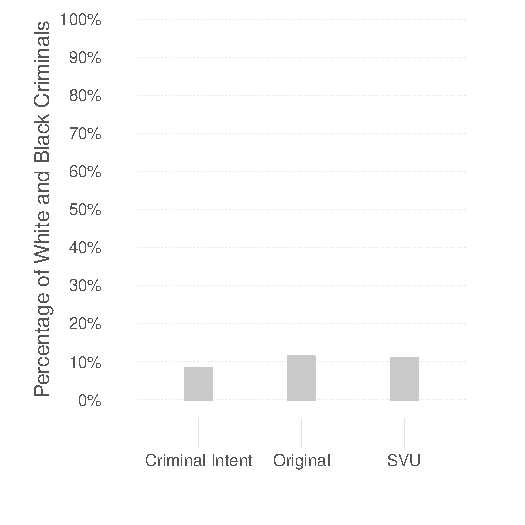
\includegraphics[scale=1]{../figs/all_criminals_by_race.pdf}
\label{fig:perp_race}
\end{figure}

Not only were the perpetrators overwhelmingly white, so were the victims (see Figure \ref{fig:victim_race}). Once again, nearly 90\% of the victims depicted in all three shows were white. Splitting the data by year and tallying percentage of victims who were white shows no discernible time trend across the shows (see Figure~\ref{fig:victim_race_ts} and Table~\ref{tab:v_race}). Compared to Law \& Order, where only about 10 percent of the victims were black, the average percentage of victims of a serious violent crime between 1999 and 2014 who were black was 19.8\%. Commensurate number for victims of sexual assault was 15.21\%, for aggravated violence, it was 19.4\%, and for murder, it was an astonishing 43\% (see Table~\ref{tab:v_race}).

\begin{figure}[htbp]
\centering
\caption{Race of Victims Across Law \& Order, SVU, and Criminal Intent}
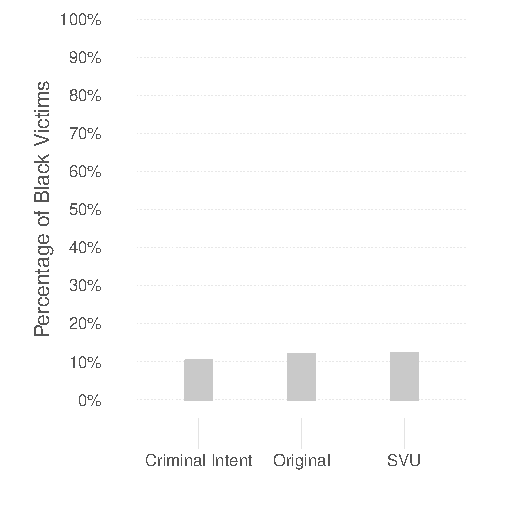
\includegraphics[scale=1]{../figs/all_victims_by_race.pdf}
\label{fig:victim_race}
\end{figure}

Moving to gender, nearly 30\% of the perpetrators were men across all the three shows (see Figure\ref{fig:perp_sex}). Once again, there is no distinct over time pattern in percentage of perpetrators who were men across the three shows (see Figure~\ref{fig:perp_sex_ts} and Table~\ref{tab:c_sex}). The percentage of female perpetrators in the real world based on arrest data is lower---ranging from 11.1\% of murderers to approximately 1.4\% of rapists to nearly 18.4\% of those arrested for a violent crime. 

\begin{figure}[htbp]
\centering
\caption{Gender of Perpetrators Across Law \& Order, SVU, and Criminal Intent}
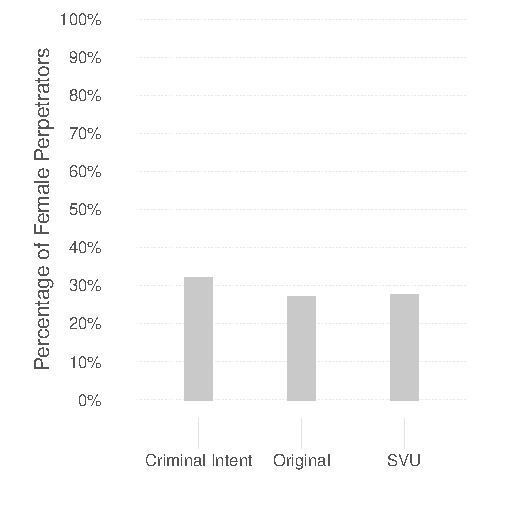
\includegraphics[scale=1]{../figs/all_criminals_by_gender.pdf}
\label{fig:perp_sex}
\end{figure}

When we looked at the gender of victims, there was an expected sizable variation across shows, with female victims constituting roughly 40\% of all the victims on CI and Original and just over 60\% on SVU. were men across all three shows (see Figure\ref{fig:victim_sex}). Except for CI, where there appears to be downward trend post 2005, there was no discernible time trends in CI and SVU (see Figure~\ref{fig:victim_sex_ts} and Table~\ref{tab:v_sex}). In the real world, percentage of victims of serious violent crime who are women is about 47\%. Percentage of female victims of rape or sexual assault is a distressing 89.2\%. And the commensurate numbers for victims of aggravated assault and murder are 40.7\% and 22.5\% approximately. 

\begin{figure}[htbp]
\centering
\caption{Gender of Victims Across Law \& Order, SVU, and Criminal Intent}
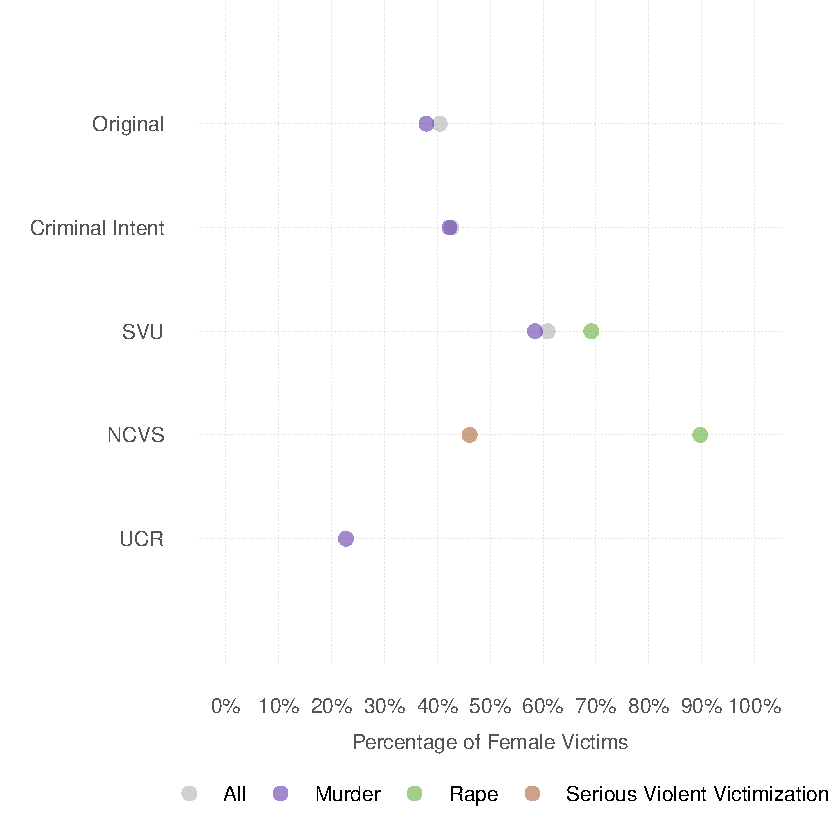
\includegraphics[scale=.9]{../figs/all_victims_by_gender.pdf}
\label{fig:victim_sex}
\end{figure}

\section*{Discussion}
Popular television is our bay window to the world. What we see on television likely has a sizable influence on how we think about various aspects of the world. In particular, television programming likely influences how we think about crime, how common we think it is, especially in our communities, who we think perpetrates it, the reasons why criminals do what they do, who the victims are, the efficacy of the police and judicial systems, among other things.\footnote{We informally collected data was efficacy and fairness of police and judicial systems. Across all three shows, police and judicial system, despite their problems, are shown to be astonishingly efficacious and fair. According to our informal estimates, well over 80\% of the cases are successfully closed. However, we do not put too much faith in our data and recommend that other researchers collect more systematic data on the point.} 

In this essay, we shed light on whether a popular police procedural perpetuates adversarial stereotypes of who commits crimes. We also look at how the race and gender of victims. In line with other evidence (see Table \ref{tab:lit}), we find that contrary to worries about overrepresentation of blacks as criminals, whites are significantly overrepresented as perpetrators, and to a smaller degree, overrepresented as victims. We also find that women are overrepresented as criminals. A naive but avid viewer of Law \& Order may mislearn that the percentage of perpetrators and victims of crime who are white is substantially higher than it is. This, in turn, may shape their views about crime and policies that are likely to be most efficacious in reducing crime.

\clearpage
\bibliographystyle{apsr}
\bibliography{crime}


\clearpage
\appendix
\renewcommand{\thesection}{SI \arabic{section}}
\renewcommand\thetable{\thesection.\arabic{table}}  
\renewcommand\thefigure{\thesection.\arabic{figure}}
\counterwithin{figure}{section}

\begin{center}
\Large{Supporting Information}
\end{center}

\section{Percentage of Black and Female Perpetrators and Victims in Law \& Order By Season}

\begin{figure}[htbp]
\centering
\caption{Race of Perpetrators Across Law \& Order, SVU, and Criminal Intent}
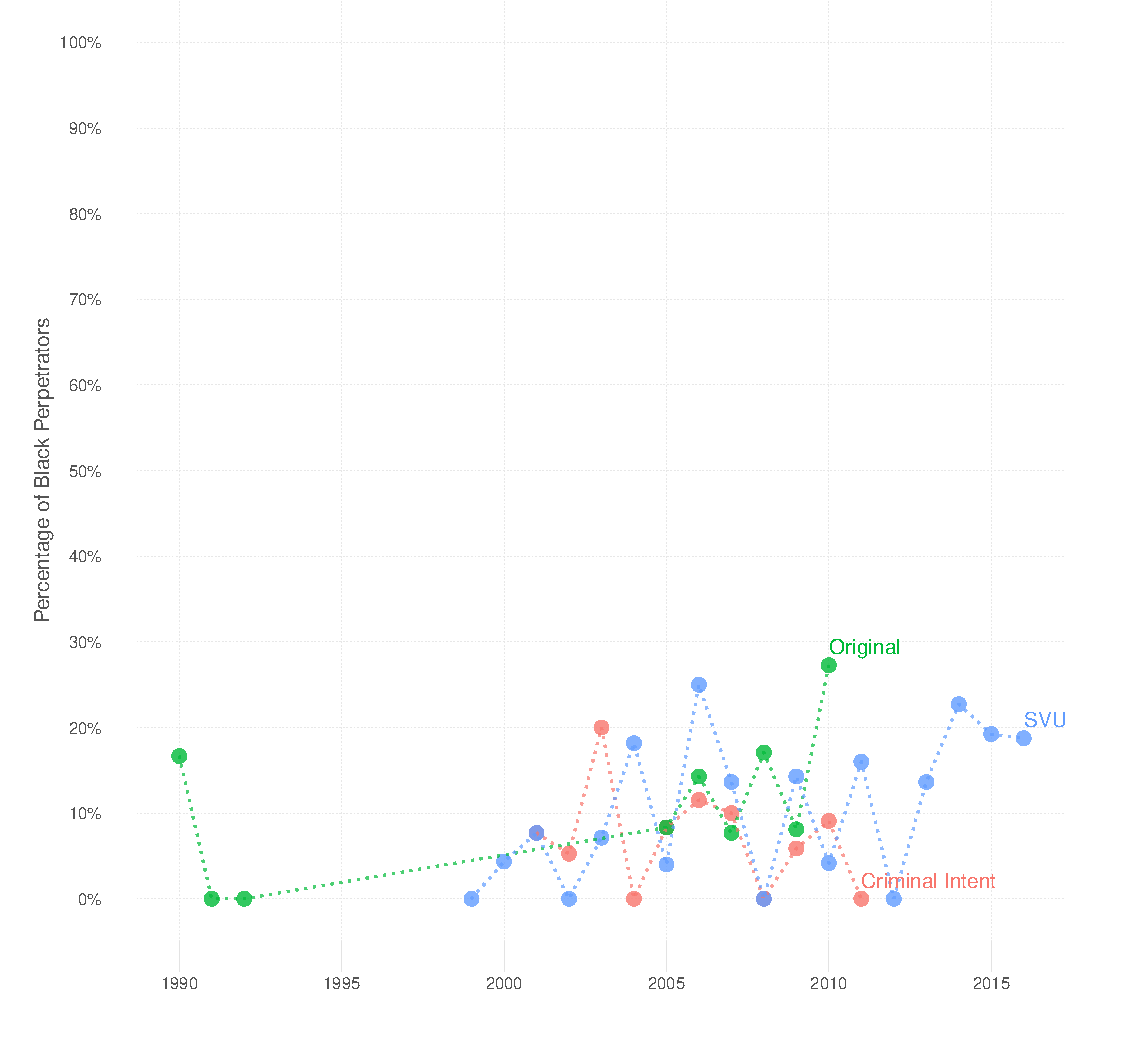
\includegraphics[scale=.9]{../figs/all_criminals_by_race_ts.pdf}
\label{fig:perp_race_ts}
\end{figure}

\begin{figure}[htbp]
\centering
\caption{Race of Victims Across Law \& Order, SVU, and Criminal Intent}
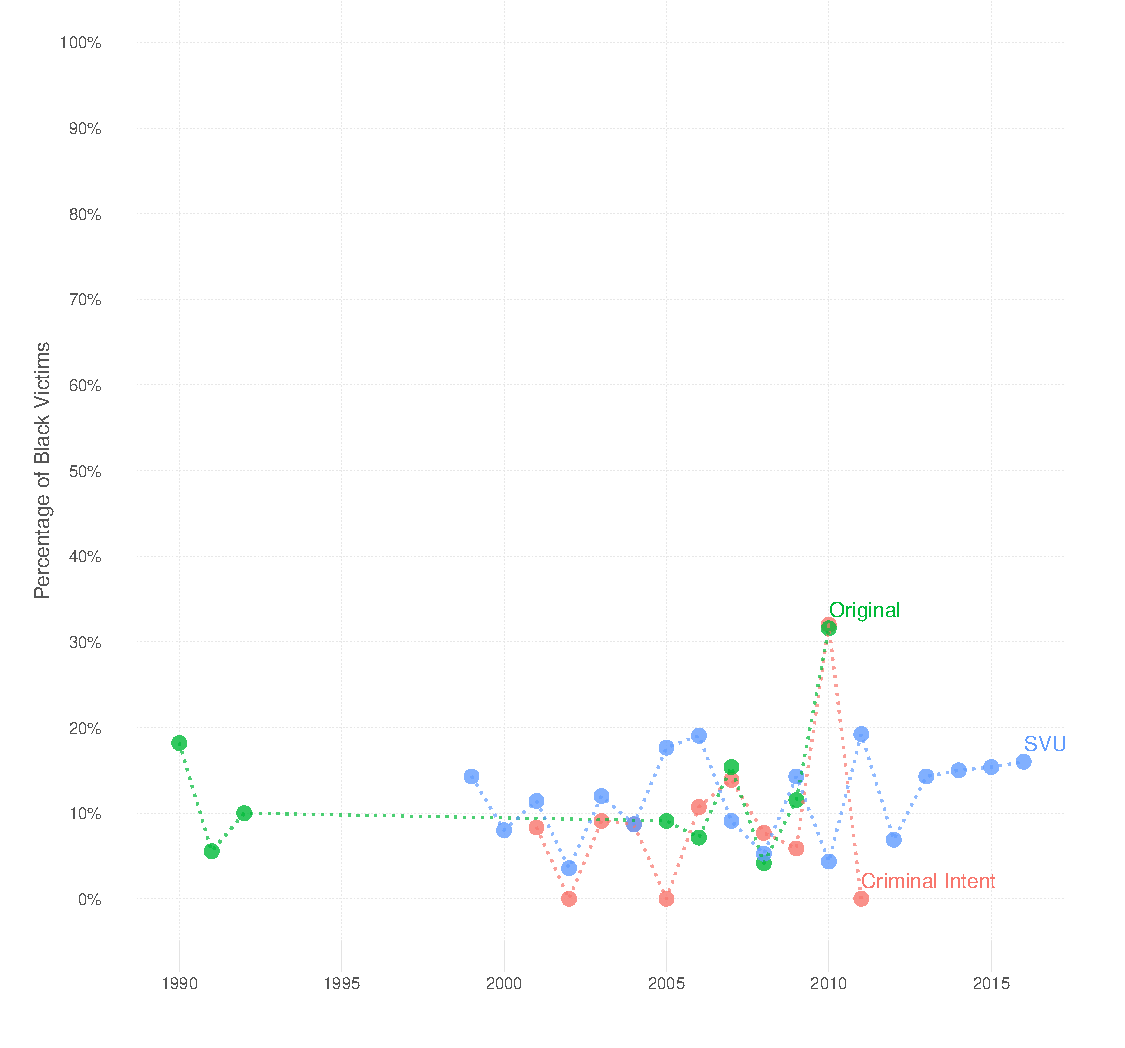
\includegraphics[scale=.9]{../figs/all_victims_by_race_ts.pdf}
\label{fig:victim_race_ts}
\end{figure}

\begin{figure}[htbp]
\centering
\caption{Gender of Perpetrators Across Law \& Order, SVU, and Criminal Intent}
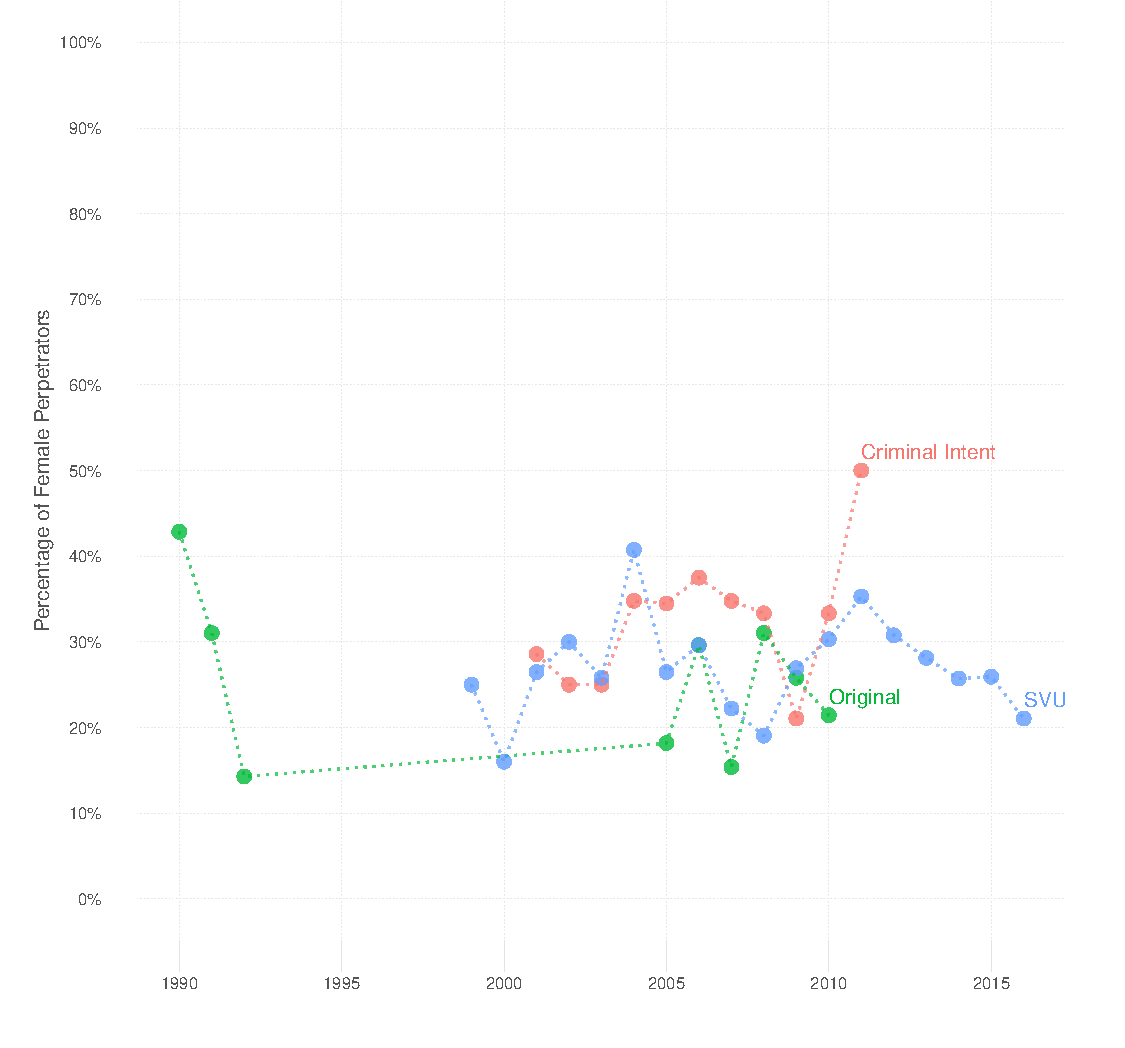
\includegraphics[scale=.9]{../figs/all_criminals_by_gender_ts.pdf}
\label{fig:perp_sex_ts}
\end{figure}

\begin{figure}[htbp]
\centering
\caption{Gender of Victims Across Law \& Order, SVU, and Criminal Intent}
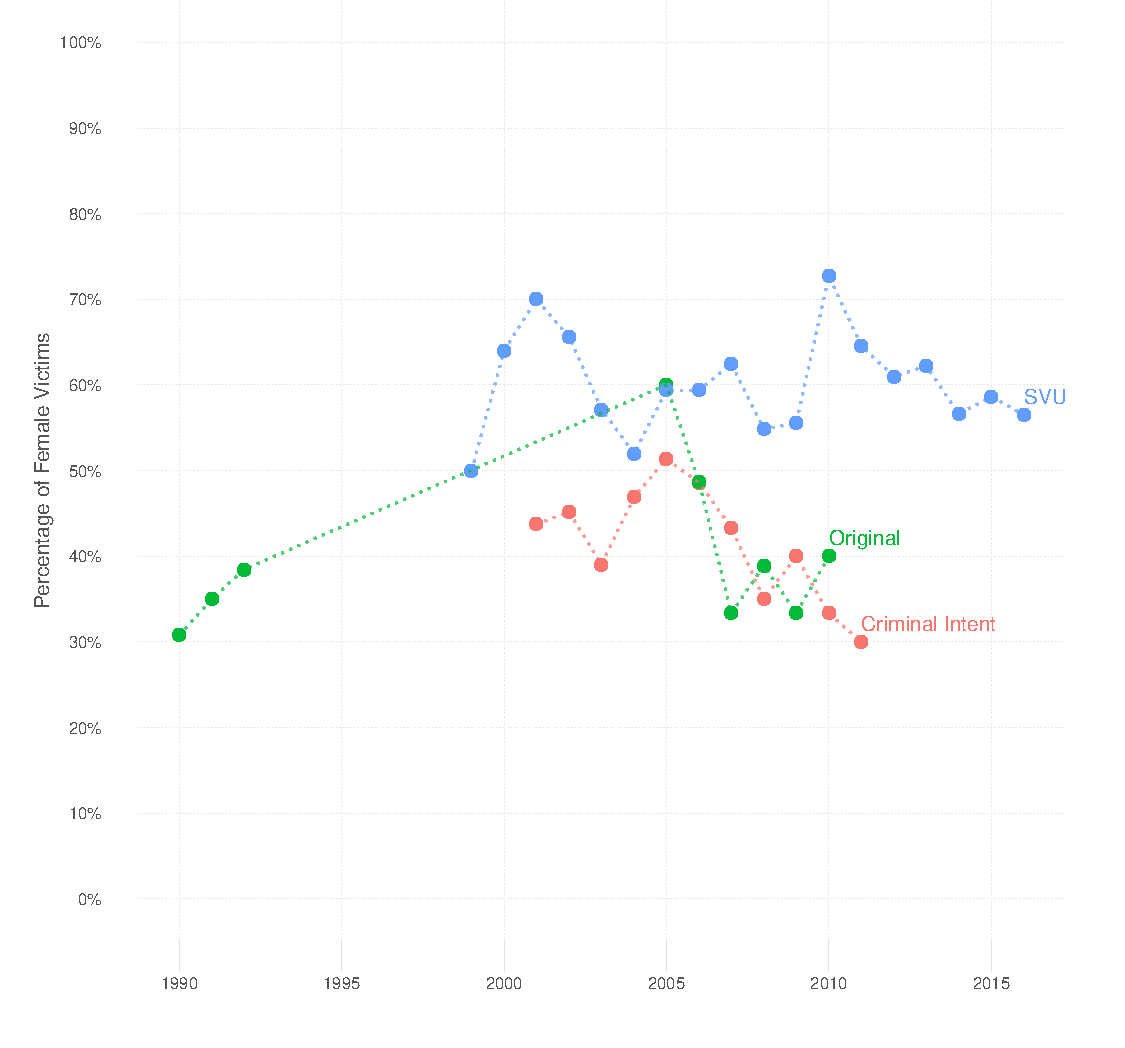
\includegraphics[scale=.9]{../figs/all_victims_by_gender_ts.pdf}
\label{fig:victim_sex_ts}
\end{figure}

\clearpage
\section{Comparison Between Sex and Race of Perpetrators and Victims in Law \& Order to the Real World}
\label{si_tabs}

% latex table generated in R 3.3.1 by xtable 1.8-2 package
% Mon Oct 10 13:56:18 2016
\begin{table}[!htb]
\centering
\caption{Percentage of Black Victims in Law \& Order, and the Real World, and Share of Blacks in the Population} 
\label{tab:v_race}
\begingroup\tiny
\begin{tabular}{cccccccccc}
  \toprule
   & \multicolumn{3}{c}{{Law and Order}} & \multicolumn{3}{c}{{NCVS}} & \multicolumn{1}{c}{{UCR}} & \multicolumn{2}{c}{{Census}}\\
 \cmidrule(lr){2-4}\cmidrule(lr){5-7}\cmidrule(lr){9-10}
 {Year} & {Criminal Intent} & {Original} & {SVU} & {Serious Violent Victimization} & {Rape or Sexual Assault} & {Aggravated Violent Victimization} & {Murder Victims} & {US} & {NY}\\
 \midrule
1990 &  & 18.2 &  &  &  &  &  & 12.0 & 28.8 \\ 
  1991 &  & 5.6 &  &  &  &  &  &  &  \\ 
  1992 &  & 10.0 &  &  &  &  &  &  &  \\ 
  1999 &  &  & 14.3 & 21.4 & 16.4 & 19.0 & 46.0 &  &  \\ 
  2000 &  &  & 8.0 & 16.0 & 9.2 & 13.8 & 48.0 & 12.3 & 26.6 \\ 
  2001 & 8.3 &  & 11.4 & 19.5 & 22.1 & 18.9 & 47.0 &  &  \\ 
  2002 & 0.0 &  & 3.6 & 22.1 & 27.3 & 22.2 & 48.0 &  &  \\ 
  2003 & 9.1 &  & 12.0 & 15.2 & 7.4 & 12.6 & 48.0 &  &  \\ 
  2004 & 8.7 &  & 8.7 & 20.0 & 19.1 & 16.7 & 47.0 &  &  \\ 
  2005 & 0.0 & 9.1 & 17.6 & 20.7 & 24.9 & 21.8 & 48.0 &  &  \\ 
  2006 & 10.7 & 7.1 & 19.0 & 21.8 & 18.9 & 27.8 & 50.0 &  &  \\ 
  2007 & 13.9 & 15.4 & 9.1 & 24.9 & 6.3 & 24.2 & 49.0 &  &  \\ 
  2008 & 7.7 & 4.2 & 5.3 & 19.2 & 16.3 & 16.4 & 48.0 &  &  \\ 
  2009 & 5.9 & 11.5 & 14.3 & 26.3 & 12.7 & 24.2 & 48.0 &  &  \\ 
  2010 & 32.0 & 31.6 & 4.3 & 19.1 & 12.2 & 21.1 & 50.0 & 12.6 & 25.5 \\ 
  2011 & 0.0 &  & 19.2 & 18.2 & 14.7 & 18.0 & 50.0 &  &  \\ 
  2012 &  &  & 6.9 & 17.9 & 5.6 & 18.6 & 51.0 &  &  \\ 
  2013 &  &  & 14.3 & 16.5 & 7.7 & 20.6 & 51.0 &  &  \\ 
  2014 &  &  & 15.0 & 17.3 & 22.6 & 15.1 & 51.0 &  &  \\ 
  2015 &  &  & 15.4 &  &  &  &  &  &  \\ 
  2016 &  &  & 16.0 &  &  &  &  &  &  \\ 
   \bottomrule
\end{tabular}
\endgroup
\end{table}


\clearpage
% latex table generated in R 3.3.1 by xtable 1.8-2 package
% Mon Oct 10 13:56:19 2016
\begin{table}[!htb]
\centering
\caption{Percentage of Black Perpetrators in Law \& Order, and the Real World, and Share of Blacks in the Population} 
\label{tab:c_race}
\begingroup\tiny
\begin{tabular}{ccccccccccc}
  \toprule
   & \multicolumn{3}{c}{{Law and Order}} & \multicolumn{5}{c}{{UCR}} & \multicolumn{2}{c}{{Census}}\\
 \cmidrule(lr){2-4}\cmidrule(lr){5-9}\cmidrule(lr){10-11}
 {Year} & {Criminal Intent} & {Original} & {SVU} & {All Crime} & {Violent Crime} & {Homicides} & {Rape} & {Assault} & {US} & {NY}\\
 \midrule
1990 &  & 16.7 &  &  &  &  &  &  & 12.0 & 28.8 \\ 
  1991 &  & 0.0 &  &  &  &  &  &  &  &  \\ 
  1992 &  & 0.0 &  &  &  &  &  &  &  &  \\ 
  1999 &  &  & 0.0 & 28.6 & 38.7 & 51.8 & 36.2 & 34.8 &  &  \\ 
  2000 &  &  & 4.3 & 27.9 & 37.8 & 48.8 & 34.1 & 34.0 & 12.3 & 26.6 \\ 
  2001 & 7.7 &  & 7.7 & 28.1 & 37.6 & 48.7 & 34.8 & 33.7 &  &  \\ 
  2002 & 5.3 &  & 0.0 & 26.9 & 38.0 & 50.0 & 34.0 & 34.2 &  &  \\ 
  2003 & 20.0 &  & 7.1 & 27.0 & 37.2 & 48.5 & 33.3 & 33.0 &  &  \\ 
  2004 & 0.0 &  & 18.2 & 26.8 & 36.9 & 47.2 & 31.9 & 32.7 &  &  \\ 
  2005 & 8.3 & 8.3 & 4.0 & 27.8 & 38.8 & 48.6 & 32.7 & 34.3 &  &  \\ 
  2006 & 11.5 & 14.3 & 25.0 & 28.0 & 39.3 & 50.9 & 32.5 & 34.5 &  &  \\ 
  2007 & 10.0 & 7.7 & 13.6 & 28.2 & 39.0 & 50.4 & 33.5 & 33.7 &  &  \\ 
  2008 & 0.0 & 17.1 & 0.0 & 28.3 & 39.4 & 50.1 & 32.2 & 34.2 &  &  \\ 
  2009 & 5.9 & 8.1 & 14.3 & 28.3 & 38.9 & 49.3 & 32.5 & 33.9 &  &  \\ 
  2010 & 9.1 & 27.3 & 4.2 & 28.0 & 38.1 & 48.7 & 31.8 & 33.5 & 12.6 & 25.5 \\ 
  2011 & 0.0 &  & 16.0 & 28.4 & 38.3 & 49.7 & 32.9 & 33.6 &  &  \\ 
  2012 &  &  & 0.0 & 28.1 & 38.5 & 49.4 & 32.5 & 34.1 &  &  \\ 
  2013 &  &  & 13.6 & 28.3 & 38.7 & 52.2 & 31.3 & 33.9 &  &  \\ 
  2014 &  &  & 22.7 & 27.8 & 37.7 & 51.3 & 29.9 & 33.1 &  &  \\ 
  2015 &  &  & 19.2 &  &  &  &  &  &  &  \\ 
  2016 &  &  & 18.8 &  &  &  &  &  &  &  \\ 
   \bottomrule
\end{tabular}
\endgroup
\end{table}


\clearpage
% latex table generated in R 3.3.1 by xtable 1.8-2 package
% Tue Oct 11 14:24:22 2016
\begin{table}[!htb]
\centering
\caption{Percentage of Female Victims in Law \& Order, and the Real World, and Share of Women in the Population} 
\label{tab:v_sex}
\begingroup\tiny
\begin{tabular}{cccccccccc}
  \toprule
   & \multicolumn{3}{c}{{Law and Order}} & \multicolumn{3}{c}{{NCVS}} & \multicolumn{1}{c}{{UCR}} & \multicolumn{2}{c}{{Census}}\\
 \cmidrule(lr){2-4}\cmidrule(lr){5-7}\cmidrule(lr){9-10}
 {Year} & {Criminal Intent} & {Original} & {SVU} & {Serious Violent Victimization} & {Rape or Sexual Assault} & {Aggravated Violent Victimization} & {Murder Victims} & {US} & {NY}\\
 \midrule
1990 &  & 30.8 &  &  &  &  &  & 51.3 & 53.2 \\ 
  1991 &  & 35.0 &  &  &  &  &  &  &  \\ 
  1992 &  & 38.5 &  &  &  &  &  &  &  \\ 
  1999 &  &  & 50.0 & 48.2 & 93.3 & 39.2 & 24.0 &  &  \\ 
  2000 &  &  & 64.0 & 38.1 & 96.0 & 27.1 & 24.0 & 50.9 & 52.6 \\ 
  2001 & 43.8 &  & 70.0 & 49.0 & 90.1 & 41.1 & 24.0 &  &  \\ 
  2002 & 45.2 &  & 65.6 & 49.3 & 86.6 & 44.0 & 23.0 &  &  \\ 
  2003 & 39.0 &  & 57.1 & 50.7 & 94.0 & 41.6 & 22.0 &  &  \\ 
  2004 & 46.9 &  & 52.0 & 45.4 & 97.6 & 37.1 & 22.0 &  &  \\ 
  2005 & 51.4 & 60.0 & 59.4 & 40.1 & 92.7 & 39.3 & 21.0 &  &  \\ 
  2006 & 48.6 & 48.7 & 59.4 & 47.4 & 77.6 & 42.5 & 21.0 &  &  \\ 
  2007 & 43.3 & 33.3 & 62.5 & 46.5 & 95.5 & 39.0 & 22.0 &  &  \\ 
  2008 & 35.0 & 38.9 & 54.8 & 54.9 & 88.7 & 47.2 & 22.0 &  &  \\ 
  2009 & 40.0 & 33.3 & 55.6 & 49.4 & 93.5 & 45.0 & 23.0 &  &  \\ 
  2010 & 33.3 & 40.0 & 72.7 & 52.5 & 94.4 & 43.2 & 23.0 & 50.8 & 52.5 \\ 
  2011 & 30.0 &  & 64.6 & 47.5 & 85.7 & 43.0 & 22.0 &  &  \\ 
  2012 &  &  & 61.0 & 42.3 & 62.2 & 42.5 & 22.0 &  &  \\ 
  2013 &  &  & 62.2 & 49.0 & 88.7 & 39.1 & 22.0 &  &  \\ 
  2014 &  &  & 56.6 & 46.9 & 90.1 & 39.6 & 23.0 &  &  \\ 
  2015 &  &  & 58.6 &  &  &  &  &  &  \\ 
  2016 &  &  & 56.5 &  &  &  &  &  &  \\ 
   \bottomrule
\end{tabular}
\endgroup
\end{table}


\clearpage
% latex table generated in R 3.3.1 by xtable 1.8-2 package
% Tue Oct 11 13:51:34 2016
\begin{table}[!htb]
\centering
\caption{Percentage of Female Perpetrators in Law \& Order, and the Real World, and Share of Women in the Population} 
\label{tab:c_sex}
\begingroup\tiny
\begin{tabular}{ccccccccccc}
  \toprule
   & \multicolumn{3}{c}{{Law and Order}} & \multicolumn{5}{c}{{UCR}} & \multicolumn{2}{c}{{Census}}\\
 \cmidrule(lr){2-4}\cmidrule(lr){5-9}\cmidrule(lr){10-11}
 {Year} & {Criminal Intent} & {Original} & {SVU} & {All Crime} & {Violent Crime} & {Homicides} & {Rape} & {Assault} & {US} & {NY}\\
 \midrule
1990 &  & 42.9 &  &  &  &  &  &  & 51.3 & 53.2 \\ 
  1991 &  & 31.0 &  &  &  &  &  &  &  &  \\ 
  1992 &  & 14.3 &  &  &  &  &  &  &  &  \\ 
  1999 &  &  & 25.0 & 21.8 & 17.0 & 11.4 & 1.3 & 19.7 &  &  \\ 
  2000 &  &  & 16.0 & 22.2 & 17.4 & 10.6 & 1.1 & 20.1 & 50.9 & 52.6 \\ 
  2001 & 28.6 &  & 26.5 & 22.5 & 17.3 & 12.5 & 1.2 & 20.1 &  &  \\ 
  2002 & 25.0 &  & 30.0 & 23.0 & 17.4 & 10.8 & 1.4 & 20.2 &  &  \\ 
  2003 & 25.0 &  & 25.8 & 23.2 & 17.8 & 10.3 & 1.3 & 20.7 &  &  \\ 
  2004 & 34.8 &  & 40.7 & 23.8 & 17.9 & 11.5 & 1.5 & 20.8 &  &  \\ 
  2005 & 34.5 & 18.2 & 26.5 & 23.8 & 17.9 & 11.0 & 1.5 & 20.8 &  &  \\ 
  2006 & 37.5 & 29.6 & 29.6 & 23.7 & 17.8 & 10.9 & 1.3 & 20.7 &  &  \\ 
  2007 & 34.8 & 15.4 & 22.2 & 24.2 & 18.2 & 10.2 & 1.1 & 21.3 &  &  \\ 
  2008 & 33.3 & 31.0 & 19.0 & 24.5 & 18.3 & 10.8 & 1.2 & 21.5 &  &  \\ 
  2009 & 21.1 & 25.8 & 26.9 & 25.3 & 18.8 & 10.4 & 1.3 & 22.0 &  &  \\ 
  2010 & 33.3 & 21.4 & 30.3 & 25.5 & 19.5 & 10.9 & 1.1 & 22.6 & 50.8 & 52.5 \\ 
  2011 & 50.0 &  & 35.3 & 25.9 & 19.6 & 11.8 & 1.2 & 22.7 &  &  \\ 
  2012 &  &  & 30.8 & 26.2 & 19.9 & 11.3 & 0.9 & 22.9 &  &  \\ 
  2013 &  &  & 28.1 & 26.5 & 20.1 & 11.7 & 1.9 & 23.0 &  &  \\ 
  2014 &  &  & 25.7 & 26.7 & 20.2 & 11.5 & 2.8 & 23.0 &  &  \\ 
  2015 &  &  & 25.9 &  &  &  &  &  &  &  \\ 
  2016 &  &  & 21.1 &  &  &  &  &  &  &  \\ 
   \bottomrule
\end{tabular}
\endgroup
\end{table}


\end{document}
